% mnras_template.tex 
%
% LaTeX template for creating an MNRAS paper
%
% v3.0 released 14 May 2015
% (version numbers match those of mnras.cls)
%
% Copyright (C) Royal Astronomical Society 2015
% Authors:
% Keith T. Smith (Royal Astronomical Society)

% Change log
%
% v3.0 May 2015
%    Renamed to match the new package name
%    Version number matches mnras.cls
%    A few minor tweaks to wording
% v1.0 September 2013
%    Beta testing only - never publicly released
%    First version: a simple (ish) template for creating an MNRAS paper

%%%%%%%%%%%%%%%%%%%%%%%%%%%%%%%%%%%%%%%%%%%%%%%%%%
% Basic setup. Most papers should leave these options alone.
\documentclass[fleqn,usenatbib]{mnras}

% MNRAS is set in Times font. If you don't have this installed (most LaTeX
% installations will be fine) or prefer the old Computer Modern fonts, comment
% out the following line
\usepackage{newtxtext,newtxmath}
% Depending on your LaTeX fonts installation, you might get better results with one of these:
%\usepackage{mathptmx}
%\usepackage{txfonts}

% Use vector fonts, so it zooms properly in on-screen viewing software
% Don't change these lines unless you know what you are doing
\usepackage[T1]{fontenc}
\usepackage{ae,aecompl}


%%%%% AUTHORS - PLACE YOUR OWN PACKAGES HERE %%%%%

% Only include extra packages if you really need them. Common packages are:
\usepackage{graphicx}	% Including figure files
\usepackage{amsmath}	% Advanced maths commands
\usepackage{amssymb}	% Extra maths symbols
\usepackage{sistyle}    %SI unit style
\usepackage{romannum}   %Roman numbering style

%%%%%%%%%%%%%%%%%%%%%%%%%%%%%%%%%%%%%%%%%%%%%%%%%%

%%%%% AUTHORS - PLACE YOUR OWN COMMANDS HERE %%%%%

% Please keep new commands to a minimum, and use \newcommand not \def to avoid
% overwriting existing commands. Example:
%\newcommand{\pcm}{\,cm$^{-2}$}	% per cm-squared

%%%%%%%%%%%%%%%%%%%%%%%%%%%%%%%%%%%%%%%%%%%%%%%%%%

%%%%%%%%%%%%%%%%%%% TITLE PAGE %%%%%%%%%%%%%%%%%%%

% Title of the paper, and the short title which is used in the headers.
% Keep the title short and informative.
\title[Running Head]{Mapping The Milky Way at 21 cm Hydrogen Line}

% The list of authors, and the short list which is used in the headers.
% If you need two or more lines of authors, add an extra line using \newauthor
\author[Mir Sakhawat Hossain et al.]{
Mir Sakhawat Hossain,$^{1}$\thanks{E-mail: s.hossain18@gmail.com}
Banrupa Mallik,$^{2}$
%Third Author$^{2,3}$
\\
% List of institutions
$^{1}$International Astrostatistics Association, Milano, Italy\\
$^{1}$Department of Mathematics, Kabi Nazrul Government College, Laxmi Bazar, Dhaka-1100, Bangladesh\\
$^{2}$Department of Physics, Begum Badrunnesa Government Women College, 7, Bakshibazar, Dhaka-1211, Bangladesh
}

% These dates will be filled out by the publisher
\date{Accepted XXX. Received YYY; in original form ZZZ}

% Enter the current year, for the copyright statements etc.
\pubyear{2018}

% Don't change these lines
\begin{document}
\label{firstpage}
\pagerange{\pageref{firstpage}--\pageref{lastpage}}
\maketitle

% Abstract of the paper
\begin{abstract}

After discovery of radiation from Galactic Hydrogen gas clouds in 1951 the 21 cm wavelength hyperfine line of atomic Hydrogen has become the best method to study spectral features in radio astronomy. It has been used as an important tracer for the distribution and velocity of gas clouds in the Inter stellar that has helped enormously to understand the galactic structure. For undergraduate level laboratory experiment it can be assembled a radio frequency receiving system at a low cost to study galactic structure. This paper presents an observation to determine the spiral structure of Milky Way galaxy which was carried out within galactic coordinate longitude $6\degr$ to $225\degr$ and latitude $0\degr$ to $35\degr$ with a low cost Haystack model type radio frequency receiving system $2.3$ metre SALSA radio telescope at Onsala Space Observatory in Sweden maintained by Chalmers University of Technology. Velocity components of Hydrogen gas clouds were calculated in different galactic longitudes and latitudes as function of distance from galactic centre to plot spiral galactic arms. This observation was made in frequency switching mode and the telescope was remotely operated by internet.
\end{abstract}

% Select between one and six entries from the list of approved keywords.
% Don't make up new ones.
\begin{keywords}
Galaxy: general -- Galaxy: structure -- radio lines: galaxies -- surveys
\end{keywords}

%%%%%%%%%%%%%%%%%%%%%%%%%%%%%%%%%%%%%%%%%%%%%%%%%%

%%%%%%%%%%%%%%%%% BODY OF PAPER %%%%%%%%%%%%%%%%%%

\section{Introduction}

Neutral Hydrogen(\ion{H}{I}) at ground state level is abundant and uniformly distributed element throughout the interstellar medium(ISM). It is the most ubiquitous element in low density regions of ISM but detectable in $\lambda\approx21$ cm or $\approx1420$ MHz where $\textnormal{H}_2$ is symmetric but not detectable at the radio frequencies. In 1933 Karl Guthe Jansky detected first extraterrestrial radio frequency\citep{jansky1933radio}. After that in 45 Then Van de Hulst predicted $21$ cm wavelength emission\citep{CJBakker1945}. The same frequency line also detected by Muller and Oort\citep{muller1951observation} in the same year. A preliminary survey was taken by Christiansen and Hindman\citep{christiansen1952preliminary} in Australia. They made this survey with a $7.5$\textnormal{-m} paraboloid and movable radio antenna with beam width between half power $1.9\degr$ in horizontal and $2.7\degr$ in vertical direction and it covered galactic longitude $-10\degr$ to $+10\degr$ at galactic plane. In Netherlands Muller and Westerhout\citep{Muller1957} took an extended neutral HI line profile survey and made a catalogue approximately in galactic latitude $\pm20\degr$ and longitude $318\degr$ to $220\degr$. Within these periods angular resolution has been developed from $30\deg$ to $30$\,-\micro as\citep{kellermann2001development,Middelberg2008}. Recently all sky mapping in HI line based on EBHIS and GASS has been completed\citep{bekhti2016hi4pi} with angular resolution $16.2\arcsec$ and sensivity $\sigma_{rms}=43$\,mK. Santo and Ashraf\citep{santo2013mapping} carried out a galactic survey to map Milky Way galaxy in galactic longitude $0\degr$ to $225\degr$ at galactic plane using SALSA radio telescope which was built for EU HOU project\citep{Doran2007}. Considering this observation we have completed our observation using the SALSA radio telescope in extended galactic coordinates i.e., galactic longitude $6\degr$ to $225\degr$ and latitude $0\degr$ to $35\degr$. We have discussed here galactic geometry for observable parameters, observation details, data analysis and results with plotting and importance of this project.

\section{Theory}

\subsection{Hyperfine Splitting of Hydrogen}

Neutral Hydrogen consists of a motionless proton(positive charged $+e$) and moving electron(negative charged $-e$) see Figure~\ref{fig:hyperfine_figure}. Electron orbits around proton for the mutual attraction of opposite charges. The derivation is as follows Griffiths\citep{griffiths2016introduction}. We can imagine electron is orbiting around nucleus(proton). From the view of electron proton is orbiting electron. This circling creates a magnetic field $\mathbfit{B}$ in the frame of electron which causes torque on spinning electron. It tends to align its magnetic moment($\bmath{\mathit{\umu}}$) along the direction of magnetic field. So Hamiltonian~(\ref{eq:hamiltonian})

\begin{equation}
  \mathit{H}=-\bmath{\mathit{\umu}\cdot\mathit{B}}
  \label{eq:hamiltonian} 
\end{equation}

\begin{figure}
 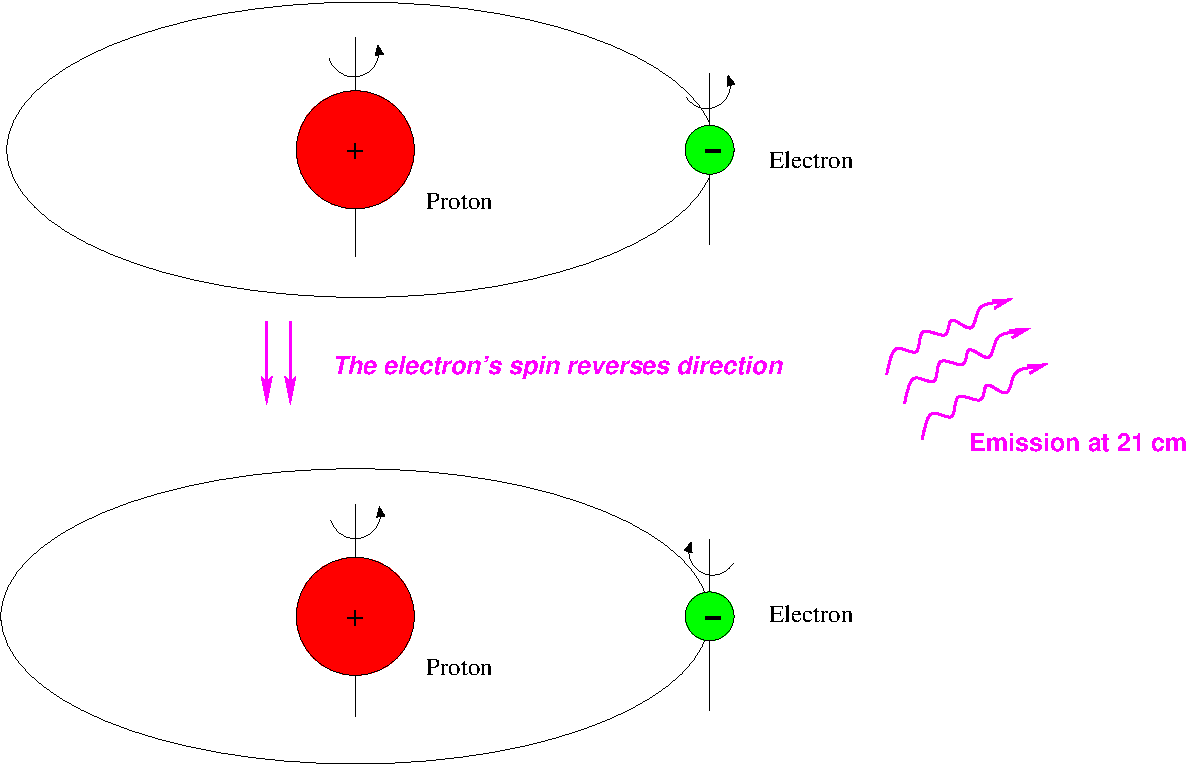
\includegraphics[width=\columnwidth]{hyperfine}
 \caption{Illustration of the 21 cm transition of the hydrogen atom, caused by the energy change
when the electron's spin changes from parallel with the proton's spin to antiparallel.}
 \label{fig:hyperfine_figure}
\end{figure}  

We can calculate magnetic field of proton($\mathbfit{B}$) and dipole moment of electron($\bmath{\mathit{\umu}}$) using Biot Savart law which is~(\ref{eq:biotsavart})

\begin{equation}
  \mathbfit{B}=\frac{\mathit{\umu_{0}I}}{2r}
  \label{eq:biotsavart}
\end{equation}

Moreover magnetic field $\mathbfit{B}$ and angular momentum $\mathbfit{L}$ is in the same direction, so~(\ref{eq:mag_ang})

\begin{equation}
 \mathbfit{B}=\frac{1}{4\upi\-\epsilon_{0}}\frac{\mathit{e}}{\mathit{mc^{2}r^{3}}}
 \label{eq:mag_ang}
\end{equation}

The direction of magnetic moment $\bmath{\mathit{\umu}}$ and spin $\mathbfit{S}$ are the same, so~(\ref{eq:mag_spin})

\begin{equation}
 \bmath{\mathit{\umu}}=\frac{\mathit{q}}{2\mathit{m}}\mathbfit{S}
 \label{eq:mag_spin}
\end{equation}

If charge of electron is $\mathit{e}$, mass of electron is $\mathit{m_{e}}$ and spin of electron is $\mathbfit{S}_{e}$ then magnetic moment of electron is~(\ref{eq:mag_electron}),

\begin{equation}
 \mathit{\bmath{\umu}}_{e}=-\frac{\mathit{e}}{\mathit{m_{e}}}\mathbfit{S}_{e}
 \label{eq:mag_electron}
\end{equation}

If mass of proton is $\mathit{m_{e}}$, spin of proton is ${\mathbfit{S}}_{e}$ and g-factor is $\mathbfit{g}_{p}$(measured value is 5.59) then magnetic moment of proton is~(\ref{eq:mag_proton}),

\begin{equation}
 \mathit{\bmath{\umu}}_{e}=\frac{\mathit{g}_{p}\mathit{e}}{2\mathit{m}_{p}}\mathbfit{S}_{p}
 \label{eq:mag_proton}
\end{equation}

In accordance with classical electrodynamics magnetic field produced by dipole $\mathit{\bmath{\umu}}$ of proton sets up magnetic field~(\ref{eq:magfield_proton})

\begin{equation}
 \mathbfit{B}=\frac{\mathit{\umu}_{0}}{4\mathit{\upi}\-\mathit{r}^{3}}[3(\mathit{\bmath{\umu}}\bmath{\cdot}\mathit{\hat{r}})\mathit{\hat{r}}-\mathit{\bmath{\umu}}]+\frac{2\mathit{\umu}}{3}\mathit{\bmath{\umu}}\mathit{\delta}^{3}(\mathbfit{r})
 \label{eq:magfield_proton}
\end{equation}

So Hamiltonian of the electron in the magnetic field due to magnetic dipole moment of proton is~(\ref{eq:dipole_proton})

\begin{equation}
\begin{split}
 \mathbfit{H}'_{hf}=\frac{\mathit{\umu}_{0}g_{p}\mathit{e}^{2}}{8\mathit{\upi}\mathit{m}_{p}\mathit{m}_{e}}\frac{[(3\mathbfit{S}_{e}\bmath{\cdot}\mathit{\hat{r}})(\mathbfit{S}_{e}\bmath{\cdot}\mathit{\hat{r}})]-\mathbfit{S}_{p}\bmath{\cdot}\mathbfit{S}_{e}}{\mathit{r}^{3}}+\\\frac{\mathit{\umu}_{0}g_{p}\mathit{e}^{2}}{3\mathit{m}_{p}\mathit{m}_{e}}\mathbfit{S}_{p}\bmath{\cdot}\mathbf{S}_{e}\delta^{3}(\mathbfit{r})
\end{split}
 \label{eq:dipole_proton}  
\end{equation}

In accordance with perturbation the first order correction is the expectation value of the perturbing Hamitonian~(\ref{eq:value_hamiltonian})

\begin{equation}
\begin{split}
 \mathit{E}_{hf}^{1}=\frac{\mathit{\umu}_{0}g_{p}\mathit{e}^{2}}{8\mathit{\upi}\mathit{m}_{p}\mathit{m}_{e}}\left\langle\frac{[(3\mathbfit{S}_{e}\bmath{\cdot}\mathit{\hat{r}})(\mathbfit{S}_{e}\bmath{\cdot}\mathit{\hat{r}})]-\mathbfit{S}_{p}\bmath{\cdot}\mathbfit{S}_{e}}{\mathit{r}^{3}}\right\rangle+\\\frac{\mathit{\umu}_{0}g_{p}\mathit{e}^{2}}{3\mathit{m}_{p}\mathit{m}_{e}}\left\langle\mathbfit{S}_{p}\bmath{\cdot}\mathbfit{S}_{e}\right\rangle\vert\mathit{\psi}\left(0\right)\vert^{2}
\end{split}
 \label{eq:value_hamiltonian} 
\end{equation}

In the ground state level the wave function is spherically symmetrical and the first expectation value vanishes. So we get~(\ref{eq:wave_function})

\begin{equation}
 \mathit{E}_{hf}^{1}=\frac{\mathit{\umu}_{0}g_{p}e^{2}}{3\upi\mathit{m}_{p}\mathit{m}_{e}\mathit{a}^{3}}\left\langle\mathbfit{S}_{p}\bmath{\cdot}\mathbfit{S}_{e}\right\rangle
 \label{eq:wave_function}
\end{equation}

This is called spin-spin coupling because of the dot product of two spin $\mathbfit{S}_{p}$ and $\mathbfit{S}_{e}$. For this coupling the individual spin angular momenta are not conserved. So the good states are eigen vectors of total spin~(\ref{eq:eigen_spin})

\begin{equation}
 \mathbfit{S}\equiv\mathbfit{S}_{e}+\mathbfit{S}_{p}
 \label{eq:eigen_spin}
\end{equation}

By applying total spin states the expected perturbation value can be written as terms of eigen operators as follows~(\ref{eq:spin_perturbation})

\begin{equation}
  \mathbfit{S}_{p}\bmath{\cdot}\mathbfit{S}_{e}=\frac{1}{2}(\mathit{S}^{2}-\mathit{S}_{e}^{2}-\mathit{S}_{p}^{2})
  \label{eq:spin_perturbation}
 \end{equation}
 
But both of electron and proton have spin $1/2$, so\\ $\mathit{S}_{e}^{2}=\mathit{S}_{p}^{2}=(3/4)\mathit{\hbar}^{2}$. In the triplet state(parallel spins) total spin is $1$ and so $\mathit{S}^{2}=2\mathit{\hbar}^{2}$. In the singlet state total spin is $0$ and $\mathit{S}^{2}=0$. Thus~(\ref{eq:total_spin})

\begin{equation}
\label{eq:total_spin}
 \mathit{E}_{hf}^{1}=\frac{4\mathit{g}_{p}\mathit{\hbar}^{4}}{3\mathit{m}_{p}\mathit{m}_{e}^{2}\mathit{c}^{2}\mathit{a}^{4}}\begin{cases}
 +\frac{1}{4}& \text{(triplet)}\\
 -\frac{3}{4}& \text{(singlet)}
\end{cases} 
\end{equation}

The spin-spin coupling breaks the spin degeneracy of the ground state lifting the triplet configuration and depressing the singlet. The energy gap is evidently~(\ref{eq:energy_gap})

\begin{equation}
 \Delta\-E=\frac{4\mathit{g}_{p}\mathit{\hbar}^{4}}{3\mathit{m}_{p}\mathit{m}_{e}^{2}\mathit{c}^{2}\mathit{a}^{4}}=5.88\times10^{-6} eV
 \label{eq:energy_gap}
\end{equation}


The frequency of the photon emitted in a transition from the triplet to the singlet state is~(\ref{eq:singlet_state}),

\begin{equation}
 \mathit{\nu}=\frac{\Delta\-E}{h}=\SI{1420}{MHz}
 \label{eq:singlet_state}
\end{equation}

The corresponding wavelength is $c/\nu=21$ cm which is part of micro wave region. In a single Hydrogen atom this transition occurs once per $\approx10^{7}$ years but enormous amount of Hydrogen in spiral arms of Milky Way galaxy causes pervasive and ubiquitous forms of radiation which is observable by radio telescope.

\subsection{Geometry of Galaxy}

The simplified geometry of the Milky Way galaxy\citep{CathyHorellou2015} see Figure.~\ref{fig:galgeo_figure}

\begin{figure}
 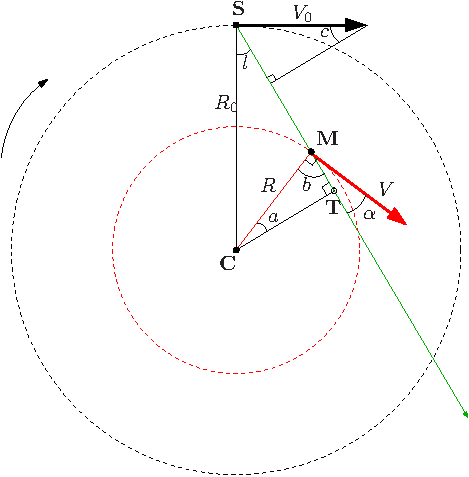
\includegraphics[width=\columnwidth]{galgeom}
 \caption{Geometry of the Galaxy. C is the location of the Galactic center, S that of the Sun, M
that of a gas cloud that we want to observe. The SM line is the line-of-sight. The arrow
on an arc indicates the direction of rotation of the Galaxy. The arrows on line segments
indicate the velocity of the Sun ($\mathbfit{V}_{0}$) and the gas cloud ($\mathbfit{V}$).}
 \label{fig:galgeo_figure}
\end{figure}

There may be many Hydrogen gas clouds in this direction, but for the purpose of this derivation we only care about a single cloud located at position M see Figure.~\ref{fig:galgeo_figure}. Since both the Sun and the cloud are moving, we do not measure the cloud velocity directly. Instead, we measure the relative velocity, $\mathbfit{V}_{r}$, between the us and the cloud, projected on the line-of-sight. Since the observation of Hydrogen gas clouds located at tangential points of galactic plane at different longitudes, the radial velocity of the gas clouds can be written as~(\ref{eq:radial_velocity}),

\begin{equation}
  \mathbfit{V}_{r}=\mathbfit{V}\cos\alpha-\mathbfit{V}_{0}\sin c
  \label{eq:radial_velocity}
\end{equation}

Where $\mathbfit{V}$ is the velocity of gas clouds and $\mathbfit{V}_{0}$ is the velocity of the Sun around galactic centre. This equation can be simplified as equation~(\ref{eq:radial_simplified}),

\begin{equation}
 \mathbfit{V}_{r}=\mathbf{V}\frac{\mathit{R}_{0}}{\mathit{R}}\sin l-\mathbfit{V}_{0}\sin l
 \label{eq:radial_simplified}
\end{equation} 

This equation is for all galactic longitude $\mathit{l}$. Here $\mathit{R}_{0}$ is distance between Sun and galactic centre, $\mathit{R}$ is distance between \ion{H}{I} gas cloud and galactic centre. We now assume that gas in Milky Way obeys differential rotation, i.e. the rotational speed is constant with radius and is the same as the rotational speed of the Sun, i.e. equation~(\ref{eq:radial_constant})

\begin{equation}
 \mathbfit{V}_{r}=Constant=\mathbfit{V}_{0}
 \label{eq:radial_constant}
\end{equation}

With this assumption we can write from equation~(\ref{eq:radial_simplified}) we can simplify as a function of cloud distance $\mathit{R}$ and $\mathbfit{V}_{r}$  as follows equation~(\ref{eq:distance_cloud})

\begin{equation}
 \mathit{R}=\frac{\mathit{R}_{0}\mathbfit{V}_{0}\sin l}{\mathbfit{V}_{0}\sin l+\mathbfit{V}_{r}}
 \label{eq:distance_cloud}
\end{equation}

From measurement of radial velocity $\mathbfit{V}_{r}$ we have calculated distance of gas cloud to the galactic centre. With the assumption of $\mathit{R}_{0}=8.5$\,kpc and $\mathbfit{V}_{0}=220$\,km\,s$^{-1}$, we can calculate value of $\mathit{R}$ for different values of galactic longitude $\mathit{l}$. From Figure.~\ref{fig:galgeo_figure} we see that in the Quadrants \Romannum{1} or \Romannum{4} there can be there may be two possible locations corresponding to given values of $\mathit{l}$ and $\mathit{R}$ to us than the tangential point T (the actual point M on the Figure.~\ref{fig:galgeo_figure}), or farther away, at the intersection of the ST line and the inner circle. But in the Quadrants \Romannum{2} or \Romannum{3} position of the emitting gas clouds can be determined uniquely\citep{CathyHorellou2015}. By the law of cosine in triangle in \textbf{CSM} we have equation~(\ref{eq:cosine_theory}),

\begin{equation}
 \mathit{R}^{2}=\mathit{R}_{0}^{2}+\mathit{r}^{2}-2\mathit{R}_{0}\mathit{r}\cos l
 \label{eq:cosine_theory}
\end{equation}

This is a second-order equation in $\mathit{r}$ where $\mathit{r}$ is distance to cloud from the Sun. The above equation has two possible solutions $\mathit{r}=\mathit{r}_{+}$ and $\mathit{r}=\mathit{r}_{-}$ that can be written as~(\ref{eq:cosine_solution})

\begin{equation}
 \mathit{r}\pm=\pm\sqrt{\mathit{R}^{2}-\mathit{R}_{0}^{2}\sin^{2} l}+\mathit{R}_{0}\cos l
 \label{eq:cosine_solution}
\end{equation}

From equation~(\ref{eq:cosine_solution}) we have discarded negative values and accepted one positive and two positive values. For convenient way of plotting to map the Milky Way structure, we convert the polar coordinate positions given as $\mathit{r}$ and $\mathit{l}$ to Cartesian $\bmath{x-y}$ coordinates using positive and negative values by~\ref{eqn:rpmtocart}

\begin{equation}
\left\lbrace
\begin{array}{l}
	x=\mathit{r} \cos (\mathit{l}-90\degr) \\
	y=-\mathit{R}_{0}+\mathit{r} \sin (\mathit{l}-90\degr) \\
\end{array}
\right.
\label{eqn:rpmtocart}
\end{equation}

Here we have deducted $\mathit{R}_{0}$ in $\bmath{y}$ values instead of adding to get image of rotation to fit the Wikipedia image of galactic coordinates and during plotting we converted values from degree to radian. By calculating the value of $\bmath{x}$ and $\bmath{y}$ for different velocities at different galactic longitudes $\mathit{l}$ in a graph to plot the map of Milky Way galaxy.

\section{Observations}

This observation was made with SALSA Radio Telescope situated in Onsala Space Observatory, Sweden. This telescope was operated to collect raw data through internet from Dhaka, Bangladesh. There are two radio lab antennas called "Brage" and "Vale". We used both of them. Each antenna has a diameter $2.3$\,-m dish. The angular resolution is $7\degr$ at \ion{H}{I} radio frequency line($\SI{1420}{MHz}$). Bandwidth of the receivers is $\SI{2.5}{MHz}$ and 256 frequency channels. Width of each channel is $\SI{9.765}{KHz}$. The telescope is controlled by qradio software. The observation was completed in frequency switching mode with reference frequency $\SI{1422.9}{MHz}$ and gain factor $800$.

\subsection{Data Reduction}

The observation was completed within galactic coordinate longitude $6\degr$ to $225\degr$ and latitude $0\degr$ to $35\degr$ following $3\degr$ for galactic longitudes and $5\degr$ for galactic latitudes. The spectra was collected with integration time $150-300$\,seconds for each. By observing radio emission from galaxy Hydrogen we come to know the motion of Hydrogen gas clouds around Milky Way galaxy. We use Doppler effect to relate observed frequency spectra to velocity of emitting Hydrogen gas clouds. By the equation of Doppler shift we get~(\ref{eq:doppler})

\begin{equation}
 \frac{\bmath{f}-\bmath{f}_{0}}{\bmath{f}_{0}}=-\frac{\mathbfit{v}}{\mathbfit{c}}
 \label{eq:doppler}
\end{equation}

Here $\bmath{f}$ is the observed frequency, $\bmath{f}_{0}$ is the rest frequency of line we are observing, $\mathbfit{v}$ is the velocity of gas clouds(positive velocity for receding and negative velocity for approaching) and $\mathbfit{c}$ is the velocity of light. Thus we converted frequency spectra to velocity scale then we corrected baselines. After that we applied Gaussian Fit function to smooth the spectra according to the equation~(\ref{eq:gaussianfit})

\begin{equation}
  \bmath{y}=\sum^n_{i=1}\bmath{a}_{i}e^{\left[-\left(\frac{\bmath{x}-\bmath{b}}{\bmath{c}_{i}} \right)^{2}\right]}
  \label{eq:gaussianfit}
\end{equation}

Here $\bmath{a}$ is the amplitude of spectra, $\bmath{b}$ is the location of the centre of peak, $\bmath{c}$ is the width of peak and $n$ is number of peaks to fit. We collected peak values with SalsaJ software and SalsaSpectrum\citep{DanielDahlin2015} MATLAB software class file. We have saved all the raw FITS files, Analysis codes, SalsaSpectrum class file and final plotted graphs in a data repository\citep{Hossain2018}.

\subsection{Result}

The Gaussian Fit equation~(\ref{eq:gaussianfit}) has been applied to calculate the central velocity of the spectra. Then we used the equation~(\ref{eq:distance_cloud}) to calculate distance $\mathit{R}$ of the clouds for different longitudes $\mathit{l}$. The values of $\mathit{R}$ has been used to calculate $\mathit{r}$ and checked whether it is single or double positive where we discarded negative values. We converted these values to the Cartesian coordinates and plotted these coordinates to unravel the spiral structure of Milky Way Galaxy using MATLAB software of version R2017a. Here Perseus arm, Orion arm and other outer arms are well detectable but some of them are merged partially. Here Map of Milky Way in Figure~\ref{fig:map-1}, \ref{fig:map-2}, \ref{fig:map-3}, \ref{fig:map-4}, \ref{fig:map-5}, \ref{fig:map-6}, \ref{fig:map-7} and \ref{fig:map-8}

\begin{figure}
      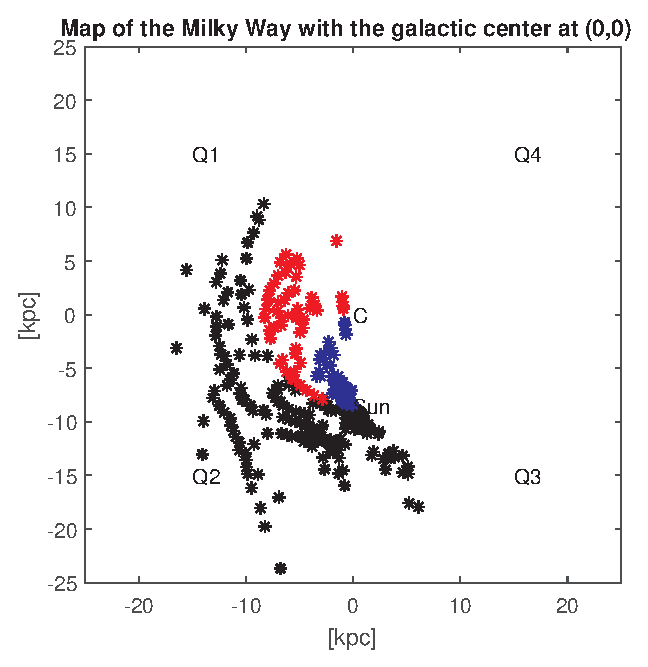
\includegraphics[width=\columnwidth]{Map_1}
      \caption{Map of Milky Way at Galactic longitude $\mathit{l}=6\degr-225\degr$ and latitude $\mathit{l}=0\degr$}
      \label{fig:map-1}
\end{figure}

\begin{figure}
      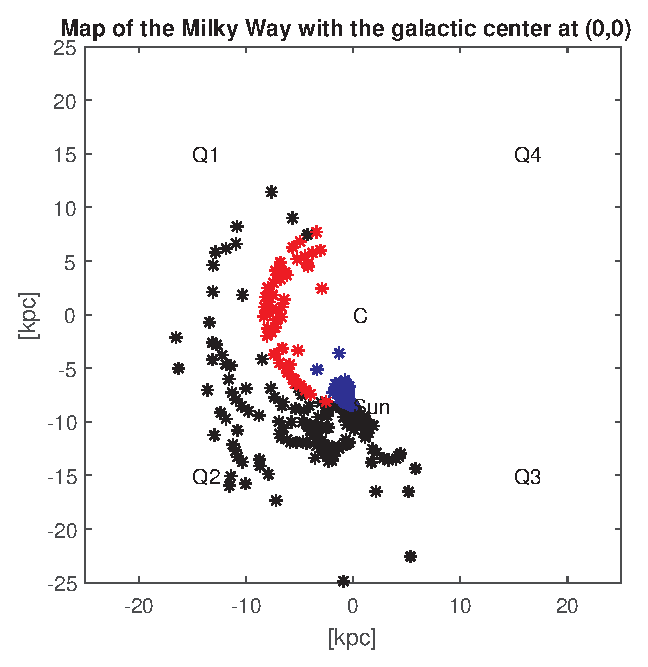
\includegraphics[width=\columnwidth]{Map_2}
      \caption{Map of Milky Way at Galactic longitude $\mathit{l}=6\degr-225\degr$ and latitude $\mathit{l}=5\degr$}
      \label{fig:map-2}
\end{figure}

\begin{figure}
      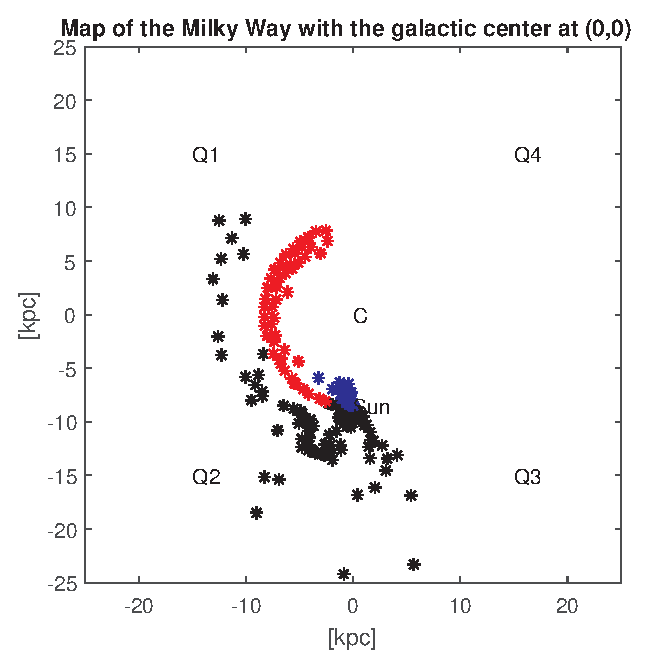
\includegraphics[width=\columnwidth]{Map_3}
      \caption{Map of Milky Way at Galactic longitude $\mathit{l}=6\degr-225\degr$ and latitude $\mathit{l}=10\degr$}
      \label{fig:map-3}
\end{figure}

\begin{figure}
      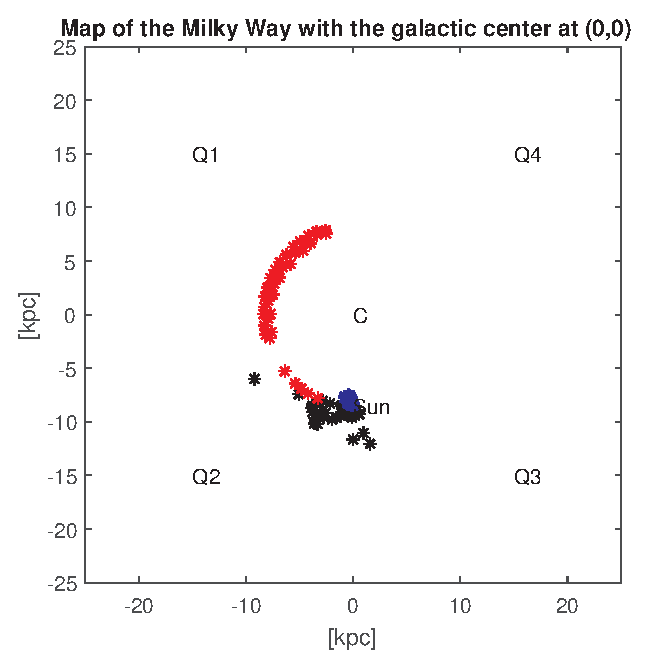
\includegraphics[width=\columnwidth]{Map_4}
      \caption{Map of Milky Way at Galactic longitude $\mathit{l}=6\degr-225\degr$ and latitude $\mathit{l}=15\degr$}
      \label{fig:map-4}
\end{figure}

\begin{figure}
      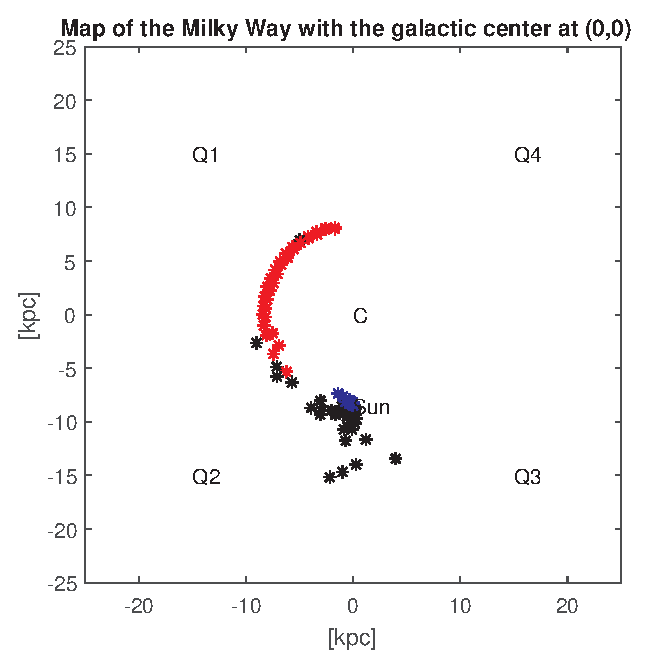
\includegraphics[width=\columnwidth]{Map_5}
      \caption{Map of Milky Way at Galactic longitude $\mathit{l}=6\degr-225\degr$ and latitude $\mathit{l}=20\degr$}
      \label{fig:map-5}
\end{figure}

\begin{figure}
      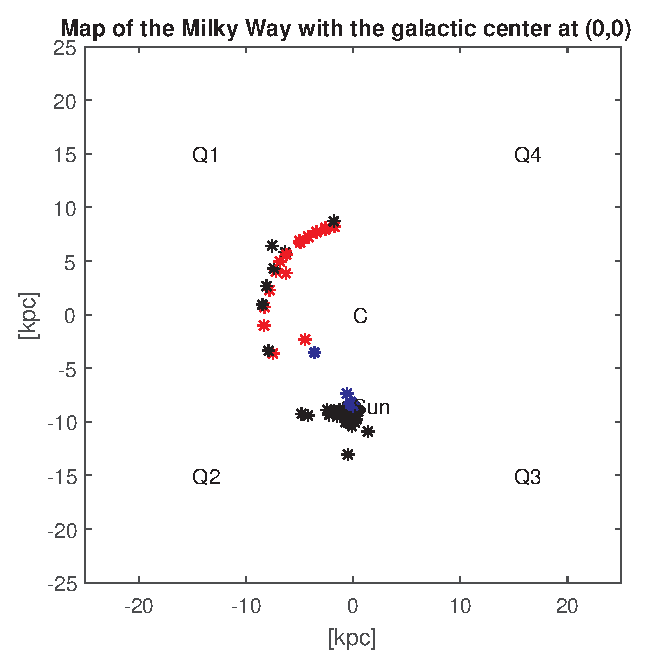
\includegraphics[width=\columnwidth]{Map_6}
      \caption{Map of Milky Way at Galactic longitude $\mathit{l}=6\degr-225\degr$ and latitude $\mathit{l}=25\degr$}
      \label{fig:map-6}
\end{figure}

\begin{figure}
      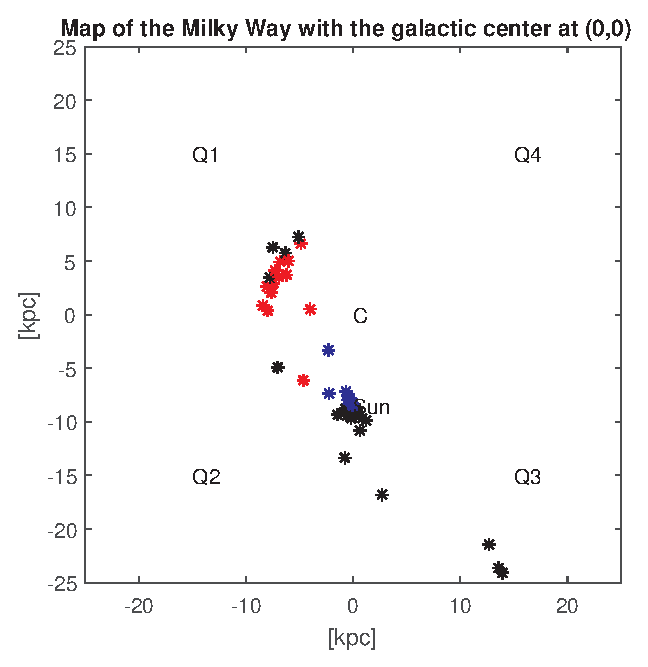
\includegraphics[width=\columnwidth]{Map_7}
      \caption{Map of Milky Way at Galactic longitude $\mathit{l}=6\degr-225\degr$ and latitude $\mathit{l}=30\degr$}
      \label{fig:map-7}
\end{figure}

\begin{figure}
      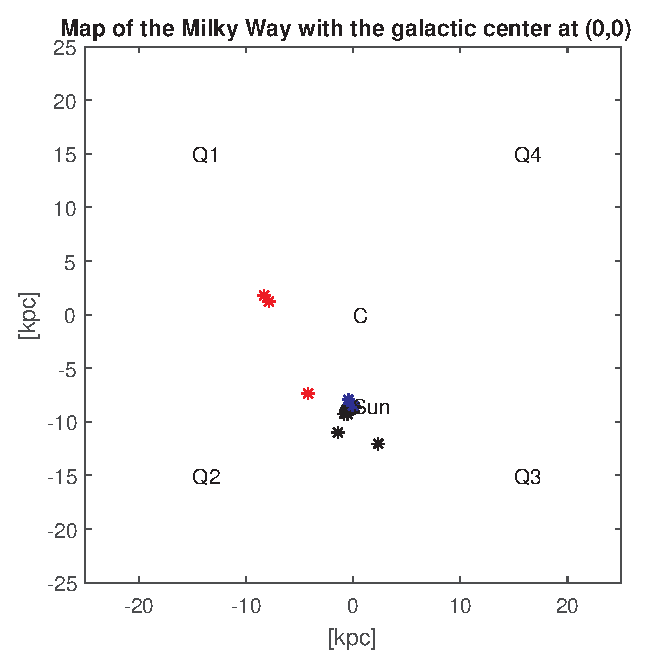
\includegraphics[width=\columnwidth]{Map_8}
      \caption{Map of Milky Way at Galactic longitude $\mathit{l}=6\degr-225\degr$ and latitude $\mathit{l}=35\degr$}
      \label{fig:map-8}
\end{figure}

Moreover we know that rotation curve is a function between circular velocity and radius. By using SALSA Telescope we can calculate the rotation curve of Milky Way. We have calculated and plotted the rotation curve see Figure~\ref{fig:rot-1}, \ref{fig:rot-2}, \ref{fig:rot-3}, \ref{fig:rot-4}, \ref{fig:rot-5}, \ref{fig:rot-6}, \ref{fig:rot-7} and \ref{fig:rot-8}. Rotation curve of most galaxies which have solar systems shows flat rotation curve i.e. $\mathbfit{V}(\mathit{R})$ does not depend on $\mathit{R}$ beyond certain radius. Angular velocity$\Omega$ varies as $\frac{1}{\mathit{R}}$. Matter near galactic center rotates with a larger angular speed than matter of farther away. But for larger radii this velocity is significantly larger than Keplerian case\citep{DanielDahlin2015}. The figures we have got indicates indirectly the existence of dark matter see Figure~\ref{fig:rot-1}, \ref{fig:rot-2}, \ref{fig:rot-3}, \ref{fig:rot-4}, \ref{fig:rot-5}, \ref{fig:rot-6}, \ref{fig:rot-7} and \ref{fig:rot-8}.

\begin{figure}
      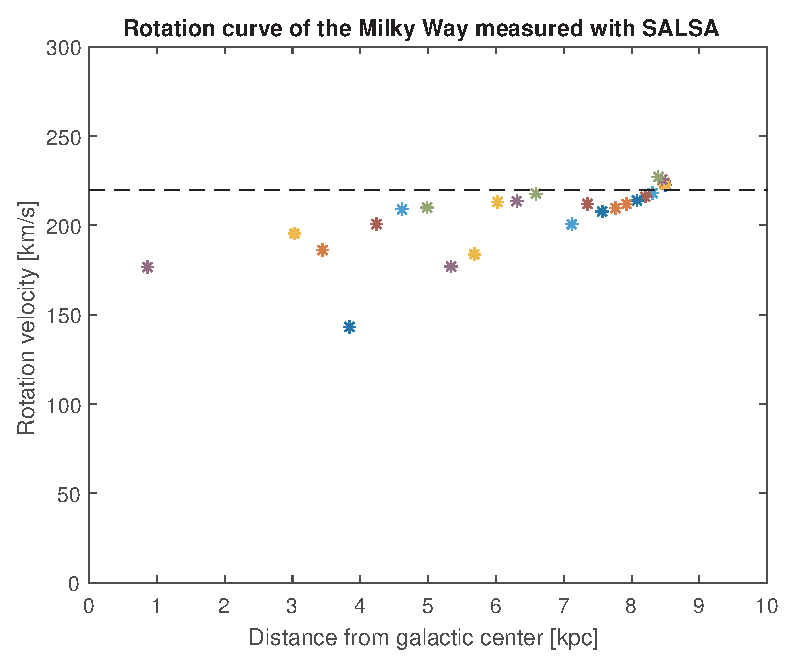
\includegraphics[width=\columnwidth]{RotationCurve_1}
      \caption{Map of Milky Way at Galactic longitude $\mathit{l}=6\degr-225\degr$ and latitude $\mathit{l}=0\degr$}
      \label{fig:rot-1}
\end{figure}

\begin{figure}
      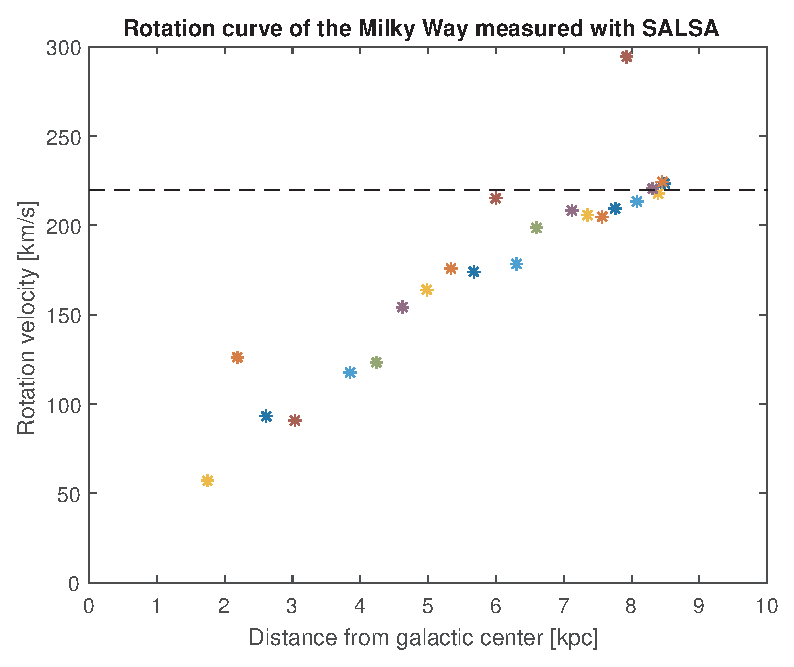
\includegraphics[width=\columnwidth]{RotationCurve_2}
      \caption{Map of Milky Way at Galactic longitude $\mathit{l}=6\degr-225\degr$ and latitude $\mathit{l}=5\degr$}
      \label{fig:rot-2}
\end{figure}

\begin{figure}
      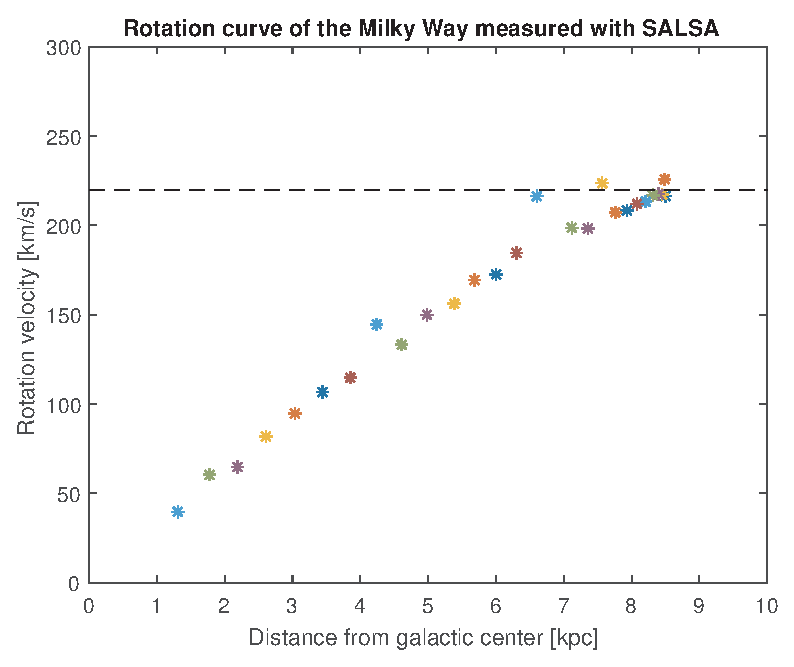
\includegraphics[width=\columnwidth]{RotationCurve_3}
      \caption{Map of Milky Way at Galactic longitude $\mathit{l}=6\degr-225\degr$ and latitude $\mathit{l}=10\degr$}
      \label{fig:rot-3}
\end{figure}

\begin{figure}
      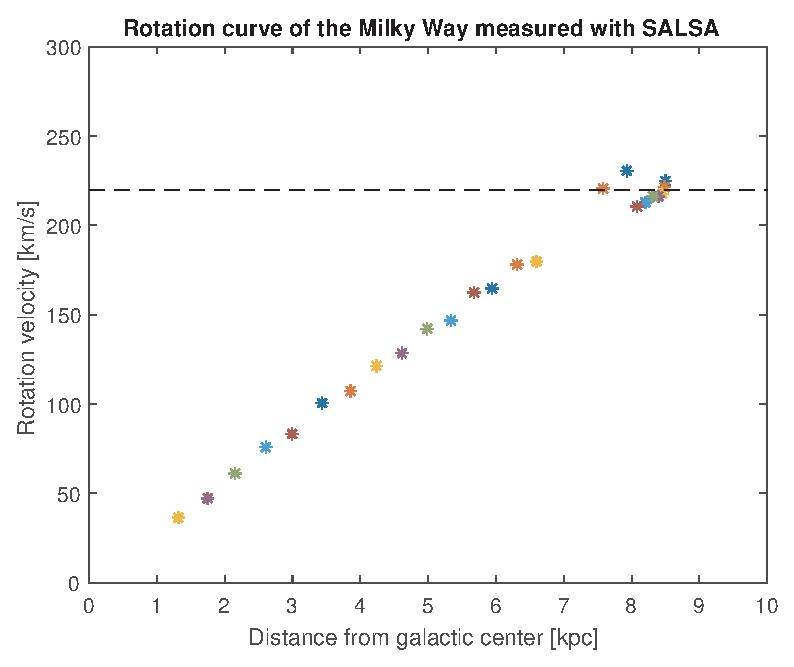
\includegraphics[width=\columnwidth]{RotationCurve_4}
      \caption{Map of Milky Way at Galactic longitude $\mathit{l}=6\degr-225\degr$ and latitude $\mathit{l}=15\degr$}
      \label{fig:rot-4}
\end{figure}

\begin{figure}
      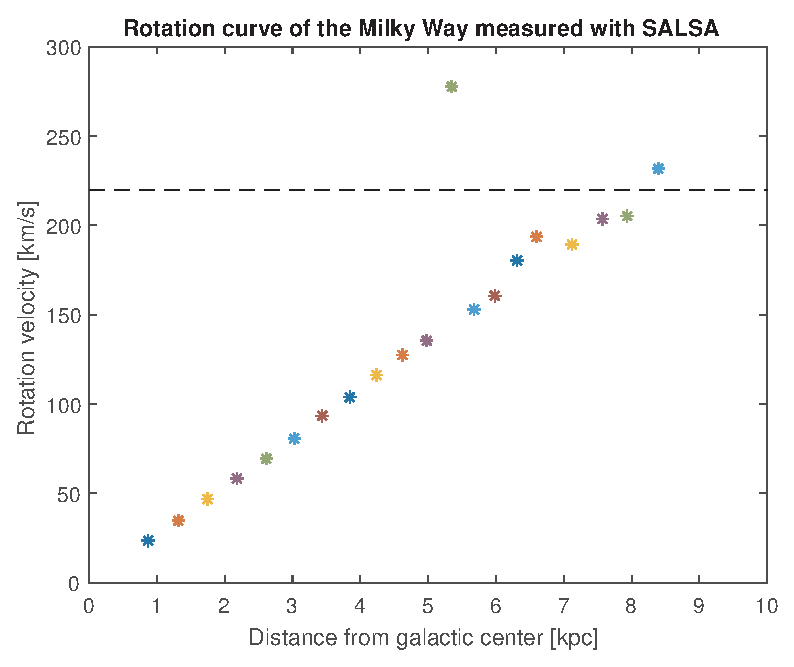
\includegraphics[width=\columnwidth]{RotationCurve_5}
      \caption{Map of Milky Way at Galactic longitude $\mathit{l}=6\degr-225\degr$ and latitude $\mathit{l}=20\degr$}
      \label{fig:rot-5}
\end{figure}

\begin{figure}
      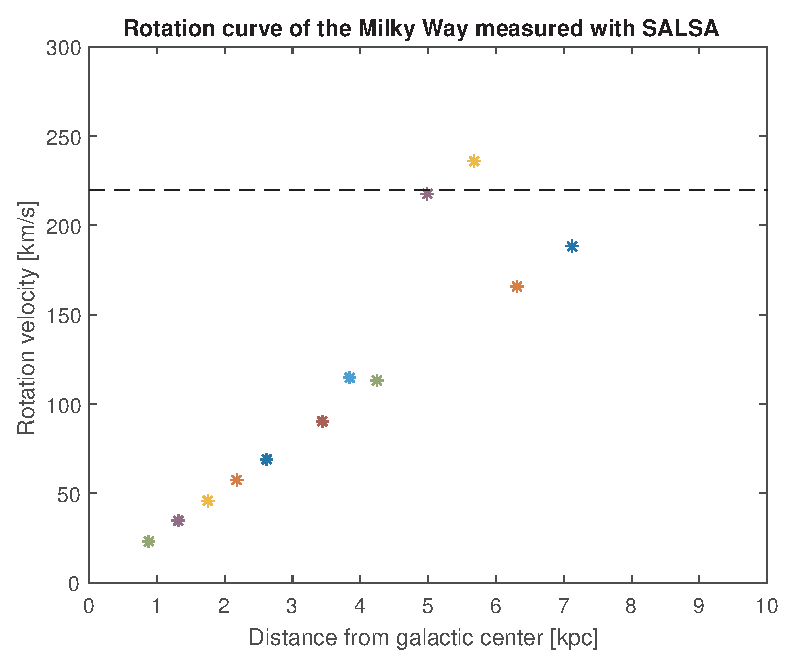
\includegraphics[width=\columnwidth]{RotationCurve_6}
      \caption{Map of Milky Way at Galactic longitude $\mathit{l}=6\degr-225\degr$ and latitude $\mathit{l}=25\degr$}
      \label{fig:rot-6}
\end{figure}

\begin{figure}
      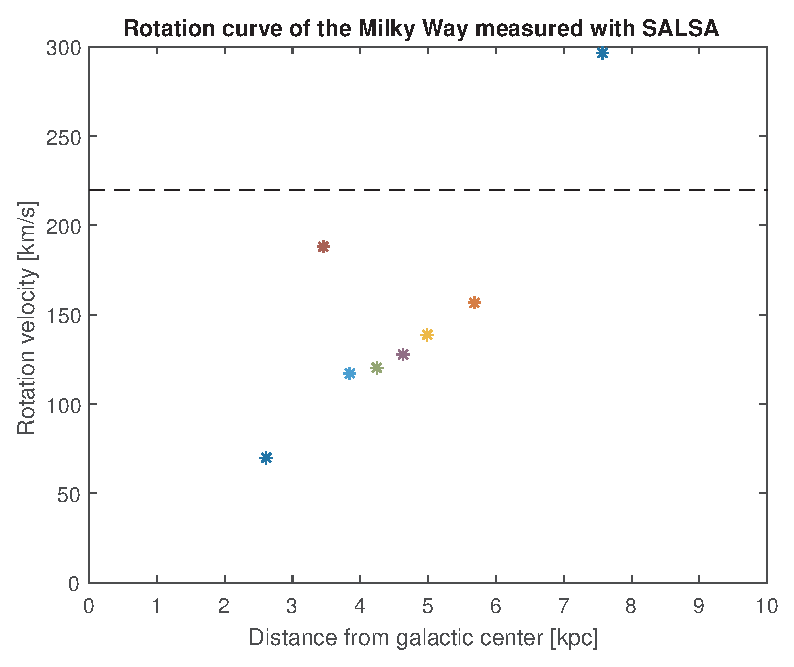
\includegraphics[width=\columnwidth]{RotationCurve_7}
      \caption{Map of Milky Way at Galactic longitude $\mathit{l}=6\degr-225\degr$ and latitude $\mathit{l}=30\degr$}
      \label{fig:rot-7}
\end{figure}

\begin{figure}
      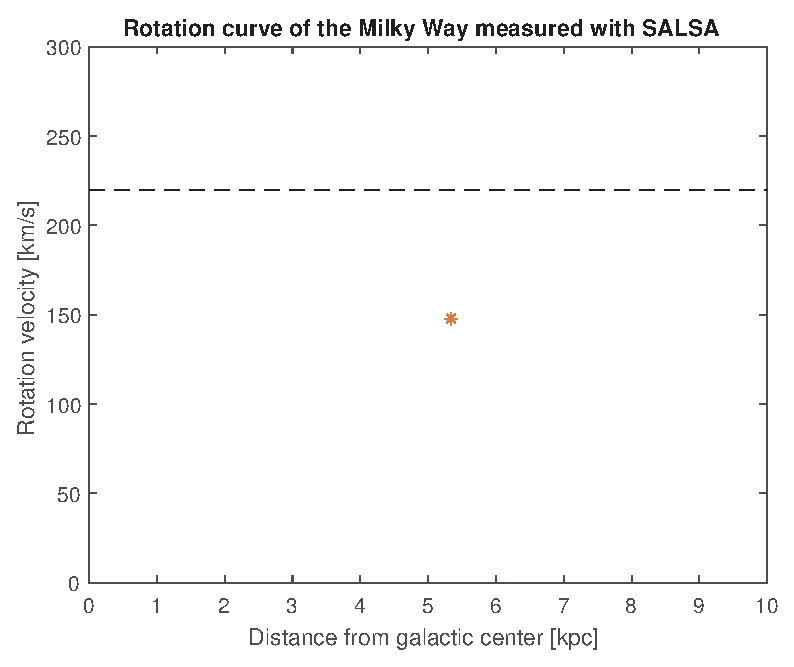
\includegraphics[width=\columnwidth]{RotationCurve_8}
      \caption{Map of Milky Way at Galactic longitude $\mathit{l}=6\degr-225\degr$ and latitude $\mathit{l}=35\degr$}
      \label{fig:rot-8}
\end{figure}

\section{Limitations and Errors}

The diameter of the SALSA Telescope is small which reduces its sensitivity. But they have strong and sensitive receiver and so detected important signals but could not detect the weaker \ion{H}{I} signals from lower density areas. Below $6\degr$ and above $225\degr$ was not possible to observe for geographical position of telescopes. Some outer arms could not be observed. There are may be errors in central velocity measurements of spectra.

\section{Importance of this Experiment}

This project is a Hands on Universe project\citep{Ferlet2006}. Here our primary goal is to show the importance of Hands on astronomy and astrophysics. This kind of practices can reduce the distance between professional astronomers and general people specially students, teachers and amateur astronomers. Cost effective instruments can be used for amateur experiments because professional observatories are tight scheduled for high level experiments. Even general people can contribute to discover new things which can be slipped by professional scientists. So this kind of experiment has importance both of education and research.


\section{Conclusions}

We have observed Milky Way galaxy within galactic longitudes $6\degr$ to $225\degr$ and latitudes $0\degr$ to $3\degr$ successfully and mapped it with rotation curves which proves the existence of dark matter. It matched with previous observations. The spiral structure is clearly detectable in maps. In future we will observe with larger professional radio telescope for all sky survey to understand the 3D structure of Milky Way and its properties with higher sensitive and higher resolution.

\section*{Acknowledgements}

We are grateful to Onsala space observatory and Chalmers University of Technology for their cooperation to complete this survey. Special thanks to Eskil Varenius who was a supervisor of SALSA who helped us a lot to operate this telescopes and provided important information.

%%%%%%%%%%%%%%%%%%%%%%%%%%%%%%%%%%%%%%%%%%%%%%%%%%

%%%%%%%%%%%%%%%%%%%% REFERENCES %%%%%%%%%%%%%%%%%%

% The best way to enter references is to use BibTeX:

\bibliographystyle{mnras}
\bibliography{mybib} % if your bibtex file is called example.bib


% Alternatively you could enter them by hand, like this:
% This method is tedious and prone to error if you have lots of references
%\begin{thebibliography}{99}
%\bibitem[\protect\citeauthoryear{Author}{2012}]{Author2012}
%Author A.~N., 2013, Journal of Improbable Astronomy, 1, 1
%\bibitem[\protect\citeauthoryear{Others}{2013}]{Others2013}
%Others S., 2012, Journal of Interesting Stuff, 17, 198
%\end{thebibliography}
% > \end{thebibliography}
%
% ^.

%%%%%%%%%%%%%%%%%%%%%%%%%%%%%%%%%%%%%%%%%%%%%%%%%%

%%%%%%%%%%%%%%%%% APPENDICES %%%%%%%%%%%%%%%%%%%%%

\appendix

\section{Some extra material}

If you want to present additional material which would interrupt the flow of the main paper,
it can be placed in an Appendix which appears after the list of references.

%%%%%%%%%%%%%%%%%%%%%%%%%%%%%%%%%%%%%%%%%%%%%%%%%%


% Don't change these lines
\bsp	% typesetting comment
\label{lastpage}
\end{document}

% End of mnras_template.tex